\documentclass[english]{article}

\usepackage{graphicx}
\usepackage{grffile}
\usepackage[T1]{fontenc}
\usepackage{babel}
\usepackage{wrapfig}
\usepackage{hyperref}

\date{\today}

\graphicspath{{Pictures/}}
\begin{document}	
	\begin{titlepage}
		\pagenumbering{gobble}
		\begin{figure}[!t]
			
\includegraphics[width=\linewidth]{up_logo.png}
		\end{figure}
		\vspace*{\stretch{1.0}}
		\begin{center}
			\huge{Project: Harvest}\\
			\large{Client: Subtrop}\\
			\vspace{10mm}
			\huge{Team: A-Cube-N}\\
		\end{center}
		\begin{center}
			\begin{tabular}{ c c c }
				Dunkley, Nathan & Grobler, Arno & Lochner, Amy \\
				\texttt{14145759} & \texttt{14011396} & \texttt{14038600}\\
				& Maree, Armand &\\
				& \texttt{12017800} &
			\end{tabular}
		\end{center}
		\begin{center}
			Department of Computer Science, University of Pretoria
		\end{center}
		\begin{center}
			\today
			\begin{figure}[!h]
				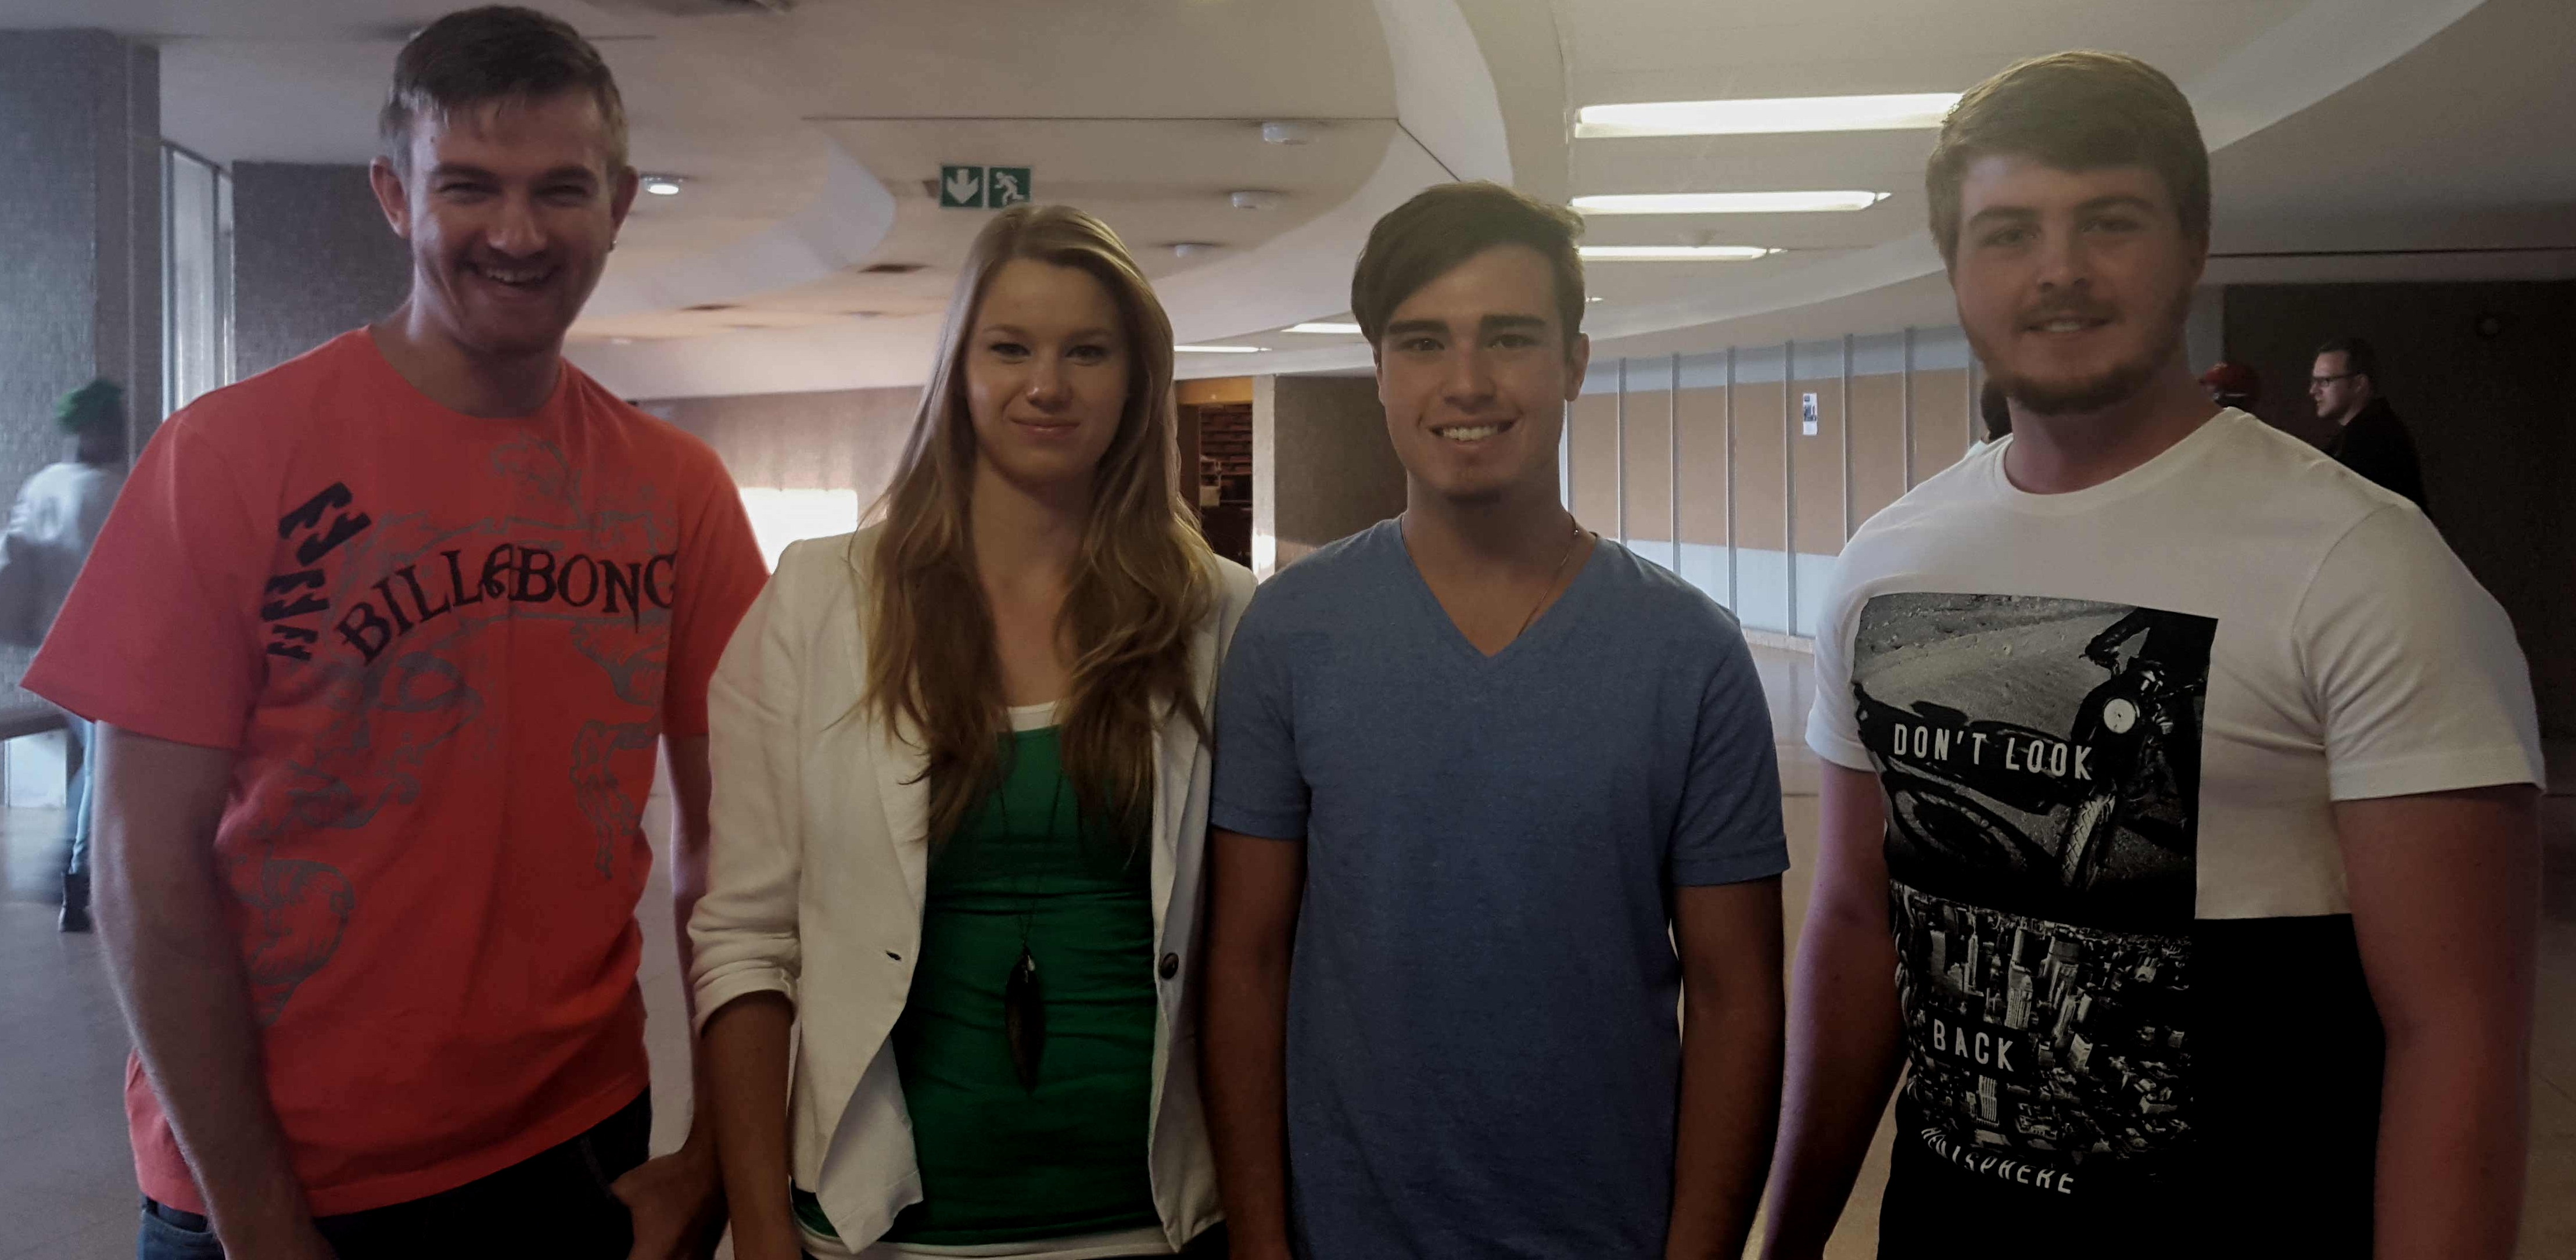
\includegraphics[width=\linewidth]{team.jpg}
			\end{figure}
		\end{center}
		\vspace*{\stretch{2.0}}
	\end{titlepage}
	\newpage
	\tableofcontents
	\newpage
	\pagenumbering{arabic}
	\section{The Team}
		\subsection{Nathan Dunkley}
		\begin{wrapfigure}{l}{5cm}
			\begin{center}
				
\includegraphics[width=8cm, height=4.5cm, angle=90]{nathan.jpg}
			\end{center}
		\end{wrapfigure}
		\paragraph{Interests and Hobbies}
		My interests include playing and watching sport, specifically motorsport (Formula One, World Endurance Championship), cricket, tennis and golf. I play tennis twice a week at a club. I also like to listen to music and read books as well as play games on PC.

		\paragraph{Technical Skills}
		I'm more of a follower than a leader and I'm good at getting on with work once the tasks have been delegated to the members of the group. I enjoy working on tasks that interest me and don't mind working long hours to get it done, once I've put my mind to it. I have some experience in multiple programming languages and I enjoy learning new skills when I can. I also enjoy solving problems.

		\paragraph{Past Experience}
		Some experience in Android Development.

		\paragraph{Non-Technical Strengths}
		\begin{itemize}
			\setlength\itemsep{0.2em}
			\item Fast Learner
			\item Willing to Learn
			\item Flexible
		\end{itemize}

		\paragraph{Motivation}
		To do..
		
		\newpage
		\subsection{Arno Gerber}
		\begin{wrapfigure}{l}{5.1cm}
			\begin{center}
				
\includegraphics[width=5cm]{arno.jpg}
			\end{center}
		\end{wrapfigure}
		\paragraph{Interests and Hobbies}
		My interests include collecting music, long distance running, painting and drawing, reading, computer games and obviously spending most of my days programming. Not only do I want to program as a profession, it is also a hobby for me. Integrating my other hobbies into my programming is my passion.
		
		\paragraph{Technical Skills}
		I pride myself in always looking for new skills and for me, learning a new technical skill is the best part of the experience. I enjoy making my projects look visually pleasing and spend as much time making a working, functional program as I do making it look good. I have good logical and problem solving skills and enjoy problems presented to me in computer science. My technical skills stem from Mathematics and computer science, especially those skills from data structures and algorithms and programming logic.
		
		\paragraph{Past Experience}
		I have created static websites for companies before, my most recent one is (\href{http://bodytalkbethlehem.com/}{http://bodytalkbethlehem.com/}) and (\href{http://honeydewpools.co.nf/}{http://honeydewpools.co.nf/}).
		
		\paragraph{Non-Technical Strengths}
		\begin{itemize}
			\setlength\itemsep{0.2em}
			\item Eager learner
			\item Organised 
			\item Good time management
			\item Good communication skills
			\item Creative
		\end{itemize}
		
		\paragraph{Motivation}
		The most appealing part of this project was the huge practical implications of having this system developed for the agricultural industry. Developing a project that a person knows is going to be used and has a use in today's world increases the motivation of the person developing the software. The technologies that were requested is also appealing as I have always wanted to make a cross platform application.
		
		\newpage
		\subsection{Amy Lochner}
		\begin{wrapfigure}{l}{5cm}
			\begin{center}
				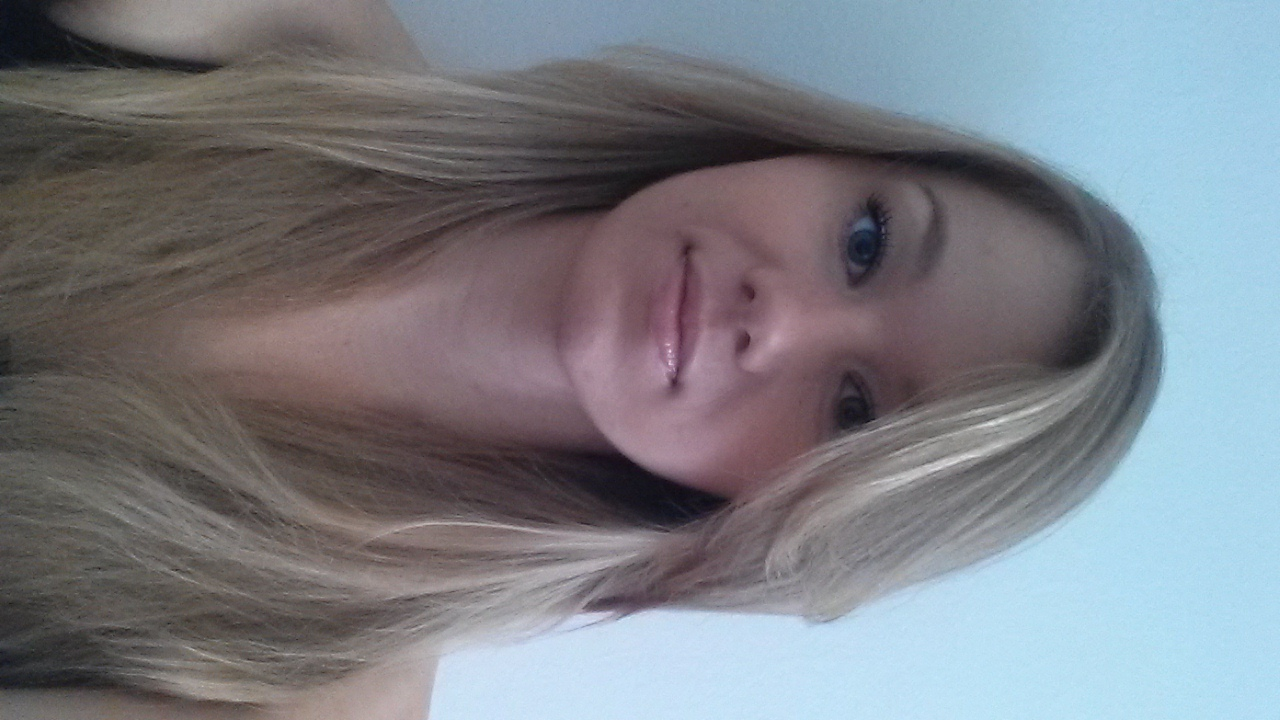
\includegraphics[width=8cm, height=4.5cm, angle=90]{amy.jpg}
			\end{center}
		\end{wrapfigure}
		\paragraph{Interests and Hobbies}
		My interests include music, classic cars, cooking, traveling, breeding Shetland sheepdogs. My hobbies include reading, playing piano, camping, 4x4ing, tennis, training my dog, mountain biking and horse riding.
		
		\paragraph{Technical Skills}
		I am good at determining functional requirements of a system. I can place myself in the users shoes, this is valuable when determining how the user will intend to use a system. I can follow business logic easily and I have experience in databasing, Informatics, Statistics, Mathematics, multiple programming languages and Human Computer Interaction.
		
		\paragraph{Past Experience}
		I have built a fully functional, responsive website. I have helped a company modify their website. I have also observed (by job shadowing) the process of creating a system for a business and have noticed which qualities have caused them to excel and which have caused them to fail. I intend to use that knowledge to keep our team constantly progressing forward.
		
		\paragraph{Non-Technical Strengths}
		\begin{itemize}
			\setlength\itemsep{0.2em}
			\item Organized
			\item Good at prioritising 
			\item Team player
			\item Good leader
			\item Optimistic
			\item Quick learner
			\item Determined
		\end{itemize}
		
		\paragraph{Motivation}
		When I first read this project proposal I took an instant liking to the project. The whole idea of modernising a management system for subtropical farmers sounded like an amazing opportunity. I especially liked the fact that no explicit technological requirements were stated; I feel that this will allow us to be very creative and provide a system best suited to the needs of the farmers. I was ecstatic to here Subtrop wished for the project to be open source; thus allowing anyone to benefit from it. I felt that showed great generosity and kindness. I know that the farming industry is possibly one of the most important industries that contribute to the economy but also contribute to society by providing natural produce. I feel many people overlook the importance of farmers, and I have had a lot of experience in Non-profit organisations -as I went to an NPO school- and I know some of the hardships and struggles that are often presented to NPOs and therefore I would feel honoured to be part of the team selected to help the farmers in Subtrop join the mobile community.
		
		\newpage
		\subsection{Armand Maree}
			\begin{wrapfigure}{l}{5.1cm}
				\begin{center}
					
\includegraphics[width=5cm]{armand.jpg}
				\end{center}
			\end{wrapfigure}
			\paragraph{Interests and Hobbies}
			During my off time I like to socialize with friends and enjoy watching sports. I also like solving puzzles to keep my brain active during holidays.\\
			Tutoring scholars and university students has become a passion for me. I always look forward to these sessions.
			
			\paragraph{Technical Skills}
			I am good at solving complex problems and building data structures. I believe this is a valuable skill to complete any project, especially in the field of computer science.
			
			\paragraph{Past Experience}
			I have developed websites for other start up companies and I also have a website of my own (\href{http://www.codehaven.co.za}{www.codehaven.co.za}). I also have some Android developing experience I gained from side projects.
			
			\paragraph{Non-Technical Strengths}
			\begin{itemize}
				\setlength\itemsep{0.2em}
				\item Good leader
				\item Fast learner
				\item Team player
				\item Good communicator
				\item Passionate
				\item Problem solver
			\end{itemize}
			
			\paragraph{Motivation}
			As soon as I read the project specifictions I was very eager to apply for it. The most attractive part of the project was the fact that is so applicable to the industry. Developing a system that would directly help the country, and more specifically farmers, sounded like a great idea. Since I am also a huge advocate of open source software, the proposal by Subtrop to make this software available for other farmers was a big attraction.
			
	\newpage
	\section{Project Execution}
		\subsection{Development Methodology}
			\paragraph\indent
			We are planning on using the Agile iterative software development methodology. The reason we have chosen this methodology can be described through the benefits of this methodology:
			\begin{itemize}
				\setlength\itemsep{0.2em}
				\item High degree of collaboration between the client and project team
				\item Allows clients to be involved throughout the project - this requires clients to understand that the work they will see is a 'work in progress'
				\item By using the idea of Sprints new features are delivered quickly and frequently
				\item Focusing on users needs results in each feature incrementally delivering value not only an IT component
				\item The breaking down of the projects into units allows the team to focus of high-quality development, testing and collaboration. Quality is improved by finding and fixing bugs quickly, and realising expectation mismatched quickly
			\end{itemize}
			
			more information on the benefits of this methodology can be found at: \sloppy\url{http://www.seguetech.com/blog/2013/04/12/8-benefits-of-agile-software-development}
			This methodology will allow us to frequently display working progress of the desired system to the client. It will also allow us to have larger, but still manageable, portions of the work done between each meeting. We believe this is essential in order to make faster progress while still being able to make changes to the system should the requirements change. See figure \ref{fig:developmentMethodologies}.
			
			\begin{figure}[!h]
				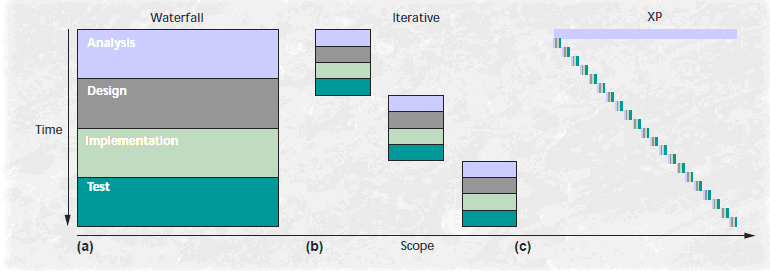
\includegraphics[width=\linewidth]{developmentMethodologies.png}
				\caption{Waterfall vs Iterative vs Extreme Programming methodologies.}
				\label{fig:developmentMethodologies}
			\end{figure}
		
		\subsection{Client Updates}
			\paragraph\indent
			Since Subtrop is located in Tzaneen it will be difficult to have frequent face-to-face meetings. As such it will be more practical have Skype/Team Viewer meetings to demonstrate the progress of the system as it stands at a particular time. Less frequent face-to-face meetings could be arranged in order for Subtrop and developers (students) to discuss important milestones in the project, should it be necessary. Regularly updates (weekly or fortnightly) can be made known to the client via email. We could make use of a tasking system in which we set a number of tasks we wish to achieve and make this available to the client in order for them to monitor our progress.
			
		\subsection{Initial Ideas}
			\paragraph\indent
			We intend to begin this project by gathering requirements from all stakeholders and doing a thorough analysis of these requirements. We will do this (hopefully in person or by means of Skype). We hope to be able to visit on site to get a feel of the work flow process and possibly discover overlooked aspects which can help us create a better Design specification. We will also determine any 'nice-to-have' aspects stakeholders may want in the system. We will then create an Analysis an Design specification which will provide the client with information regarding
			\begin{itemize}
				\item Access channel requirements
				\item Quality requirements
				\item Integration requirements
				\item Architecture constraints
				\item Use Case prioritization
				\item Required functionality depicted by use cases
				\item Process specification (more detailed steps of a use case)
				\item Domain Model
				\item Open issues we may have discovered
			\end{itemize}
			this document will be provided to Subtrop to ensure that our plans for the software encorporate all the aspects they want in the system. Any feedback from Subtrop regarding the above mentioned aspects will be incorporated into our design specification. We will also supply subtrop with a document regarding software architecture specifications. Any feedback on this will also be incorporated in the specification.\\

			We will then create a list of milestones to be achieved throughout this project with deadlines by which we hope to achieve these milestones. Some initial ideas regarding these milestones may be:
			\begin{itemize}
				\item Deciding on a database type
				\item Determining a database structure
				\item Creating a Design for the Graphical User Interface
				\item Creating a Web interface
				\item ....Add items here...
			\end{itemize}
		
			\subsection{Potential Technologies}
				\paragraph\indent
				    		\begin{itemize}
	    		        \item   Git and GitHub: A distrabutive version control system that is easy to use and free. It will be used to store and control the code written for the project and thus all code written by group memebers will be easily managed. (http://github.com/). 
	    		        \item PostgreSQL: Since we need to have a data store, we could use a PostgreSQL database to store the data.It is a free, open-source, cross-platform, object-orientated database management system. (http://www.postgresql.org/about/). An added benefit is the fact that it has an unlimited database size unlike many other similar technologies.
	    		        \item HTTPS: This technology is almost a must as it will increase the systems security by adding needed encryption.
	    		        \item Bootstrap: This technology is a powerful mobile first front-end framework for faster and easier web development. It will standardize the way content is displayed for the web front end.
	    		        \item SMTP: An extra for the requirements, but something that could be integral, is the protocol needed to send emails such as notifations and reminders to staff or workers.
	    		        \item JavaScript/JQuery: Used for client side functionality for example verification of user data and passwords
	    		        \item Glassfish Server:  Reference implementation of Java EE and as such supports EJB, JPA, JavaServer Faces, JMS, RMI, JavaServer Pages, servlets, etc. 
	    		        \item  JUnit Testing: A unit testing framework for the Java programming language.
	    		        \item ART and Dalvik: Android runtime (ART), is needed to compile android source code and run byte code generated from Dalvik.
	    		        \item  Xcode 7.0 and iOS SDK 9.0: Both needed to develop IOS applications
	    		    \end{itemize}
		
		\subsection{Deliverables}
			\paragraph\indent
			 After the completion of the system A-Cube-N will have a number of deliverables for Subtrop. These deliverables include:
		    \begin{itemize}
		        \item a web interface
		        \item an Android application
		        \item an iOS application
		        \item detailed documentation of the system - to facilitate any future developments
		       	\item a set of instructions to inform a user on how to install and set up the system.
		        \item a user manual that provides detailed instructions on how to use of the system in the most efficient and effective way 
		        
		    \end{itemize}
\end{document}
